\frenchspacing
\documentclass{amsart}
\usepackage{amssymb}
\usepackage{fancyhdr}
\usepackage{bbm}
\usepackage{enumerate}
\usepackage{graphicx}
\usepackage{tikz}
\usepackage{hyperref}
\pagestyle{fancy}
\usepackage[margin=1in]{geometry}
\newgeometry{left=1.5cm, right=1.5cm, top = 1.5cm}
\fancyhfoffset[E,O]{0pt}
\allowdisplaybreaks


\rhead{Andrew}   %% <-- your name here
\chead{Bessel Process and Hedging}  %% <-- update title here ***
\cfoot{\thepage}
\lhead{\today}



%% your macros -->
\newcommand{\nn}{\mathbb N}    %% naturals
\newcommand{\zz}{\mathbb Z}    %%integers
\newcommand{\rr}{\mathbb R}    %% real numbers
\newcommand{\cc}{\mathbb C}    %% complex numbers
\newcommand{\ff}{\mathbb F}
\newcommand{\qq}{\mathbb Q}
\newcommand{\cA}{\mathcal{A}}
\newcommand{\cP}{\mathcal{P}}
\newcommand{\cN}{\mathcal{N}}
\newcommand{\cM}{\mathcal{M}}
\newcommand{\cB}{\mathcal{B}}
\newcommand{\limn}{\lim_{n \to \infty}} %%lim n to infty shorthand
\newcommand{\va}{\mathbf{a}}
\newcommand{\vb}{\mathbf{b}}
\newcommand{\vc}{\mathbf{c}}
\newcommand{\vx}{\mathbf{x}}
\newcommand{\vy}{\mathbf{y}}
\newcommand{\vv}{\mathbf{v}}
\newcommand{\vw}{\mathbf{w}}
\newcommand{\vu}{\mathbf{u}}
\DeclareMathOperator{\var}{Var}  %% variance
\DeclareMathOperator{\Aut}{Aut}
\DeclareMathOperator{\Sym}{Sym}
\DeclareMathOperator{\Cov}{Cov}
\newtheorem{theorem}{Theorem}
\theoremstyle{definition}
\newtheorem{definition}{Definition}
\newtheorem{exercise}{Exercise}[section]


\begin{document}
\noindent
Bessel Process and Hedging   \hfill \today  %% <-- Update Notes here ***
\smallskip
\hrule
\smallskip
\noindent
By {\bf Andrew Lys} \qquad   %% <-- your name here ***
  {\tt alys(at)n.e}      %% <-- your uchicago email address here ***

\section{Bessel Process}
A common object of study is the Bessel process, which is the norm of an $n$-dimensional Brownian motion. 
To study its law, we may na\"ively apply It\^o's lemma to the function $f(x) = \|x\|$. Letting $R_t = \|B_t\|$, we have:
\begin{equation*}
  \mathrm{d} R_t = \frac{B_t \cdot \mathrm{d} B_t}{R_t} + \frac{n - 1}{R_t} \mathrm{d}t
\end{equation*}
This is not immediately justified, since $f$ is not twice differentiable at the origin, however, it's not hard to show, with a mollification argument, that this is indeed correct. 

So let's na\"ively apply this to $n = 1$. Then we have:
\begin{equation*}
  |B_t| = \int_0^t \mathrm{sgn}(B_s) \mathrm{d} B_s 
\end{equation*}
But this is wrong! We will see how this is wrong, but a quick simulation shows that the two sides are not equal:
\begin{center}
  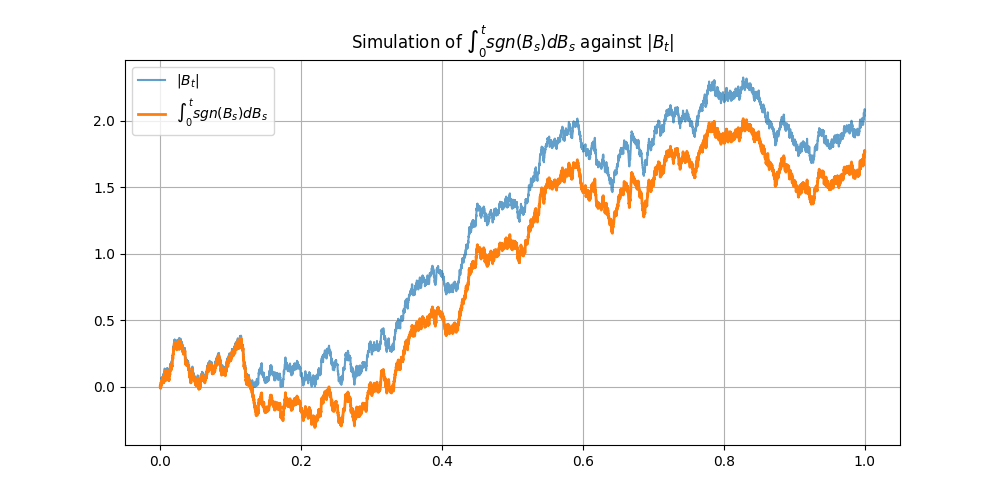
\includegraphics[width=\textwidth]{abs(Bt) vs int sign(Bt)dBt.png}
\end{center}
To solve this, we introduce the concept of local time. 
Intuitively, local time is a stochastic process that measures how much time another stochastic process spends at a particular point. 
We consider Brownian motion, and are interested in the quantity 
\[
L_t(x) = \lim_{\epsilon \downarrow 0} \frac{1}{2\epsilon}\int_0^t [B_s \in (x - \epsilon, x + \epsilon)]\mathrm{d} s
\]
Which, if the integrand were continuous, this would exist.
The indicator function is not very regular, so we look at $f \in C_2(\rr)$, and investigate
\[
\frac12 \int_0^t f(B_s) \mathrm{d} s = \int_\rr f(x) L_t(x) \mathrm{d} x
\]
If we stare at It\^o's lemma for a while, we see that the second derivative term is suspiciously similar to the left hand side of the above integral, if we have some function $F$ such that $F'' = f$.
A neat trick is to let 
\[
F(x) = \int_\rr f(y) (x - y)^+ \mathrm{d} y
\]
(which is also a portfolio of call options with strike $y$). 
By It\^o's lemma, we have
\begin{align*}
  \mathrm{d} F(B_t) &= \int_{-\infty}^{B_t} f(y) \mathrm{d} y \, \mathrm{d} B_t + \frac{1}{2} f(B_t) \mathrm{d} t\\
  F(B_t) &= F(B_0) + \int_0^t \int_\rr f(y) [B_s > y] \mathrm{d} y \, \mathrm{d} B_s + \frac{1}{2} \int_0^t f(B_s) \mathrm{d} s\\
  &= F(B_0) + \int_\rr f(y) \int_0^t [B_s > y] \mathrm{d} B_s \, \mathrm{d} y + \frac{1}{2} \int_0^t f(B_s) \mathrm{d} s\\
  \implies \int_0^t f(B_s) \mathrm{d} s &= 2 \int_\rr f(y) \left(
    (B_t - y)^+ - (B_0-y)^+ - \int_0^t [B_s > y] \mathrm{d} B_s
  \right) dy
\end{align*}
Which follows if you believe in a stochastic version of Fubini's theorem. 
This motivates Tanaka's formula:
\[
L_t(x) = (B_t - x)^+ - (B_0 - x)^+ - \int_0^t [B_s > x] \mathrm{d} B_s
\]

So now, how does this help us? The following argument can be completed as an exercise, but considering the mollification of $f(x) = |x|$ with
\[
g_\epsilon(x) = 
\begin{cases}
  \frac{x^2}{2\epsilon} + \frac{\epsilon}{2}& |x| \leq \epsilon\\
  |x|  & |x| > \epsilon
\end{cases}
\]
We can use It\^o's lemma on $g_\epsilon$ and apply our local time result to obtain the following:
\begin{align*}
  g_\epsilon(B_t) - g_\epsilon(B_0) &= \int_0^t g_\epsilon'(B_s) \mathrm{d} B_s + \frac12 \int_0^t g_\epsilon''(B_s) \mathrm{d} s\\
  &= \int_0^t g_\epsilon'(B_s) \mathrm{d} B_s + \int_\rr g''_\epsilon(x) L_t(x) \mathrm{d} x\\
  &= \int_0^t g_\epsilon'(B_s) \mathrm{d} B_s + 2 \int_{-\epsilon}^\epsilon \frac{1}{2\epsilon} L_t(x) \mathrm{d} x\\
\end{align*}
Taking limits, we obtain Tanaka's formula for absolute value:
\[
|B_t| = \int_0^t \mathrm{sgn}(B_s) \mathrm{d} B_s + 2 L_t(0)
\]
A quick simulation shows that this is indeed correct:
\begin{center}
  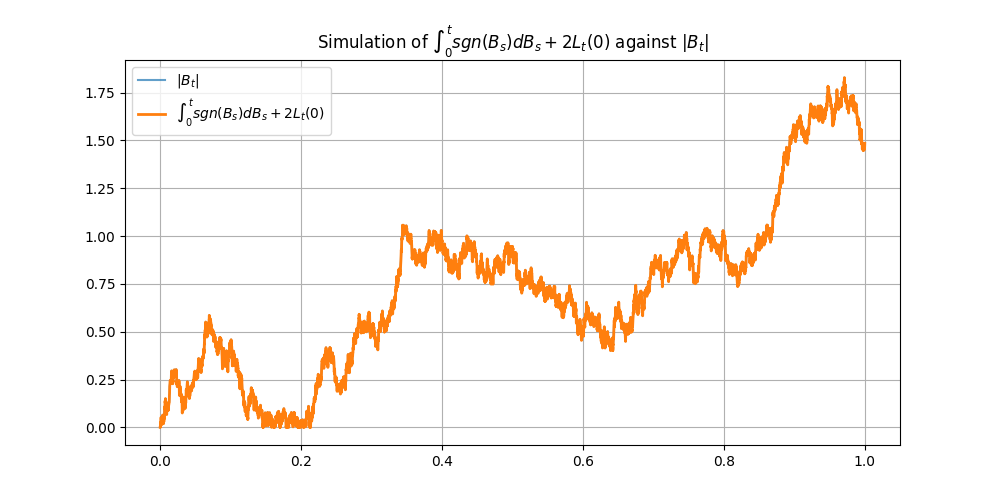
\includegraphics[width=\textwidth]{abs(Bt) vs int sign(Bt)dBt + 2Lt.png}
\end{center}
We've covered the first half of the title, now onto the second half: hedging. What does any of this have to do with hedging?

\section{Hedging}
This section is inspired by George Lowther's blog \href{https://almostsuremath.com/2023/11/07/intwge0dw/}{almost sure math}.

Let's consider a European call option with strike $K$ and expiry $T$, and lets assume this call is out of the money, i.e. $S_0 < K$. 
A hedge is a trading strategy on the underlying asset that replicates the payoff of the option at expiry. 

A na\"ive hedge for a European call option is to hold one unit of the underlying asset if the asset price is at least $K$, and hold nothing otherwise.
By this strategy, the value of the porfolio at time $T$ is $(S_T - K)^+$, which is exactly the payoff of the call option.

An immediate probelm with this strategy is that it presents an arbitrage opportunity! 
We buy for $K$, and if it drops below $K$, we lose no money, and if the stock stays above $K$ we make $(S_T - K)^+$. 
The issue is that we are requiring the trader to make uncountably many trades. 
More precisely, the stock price process has unbounded variation, so if $X_t$ is our PnL process, we do not have
$
X_T = (S_T - K)^+
$.
However, we can fix this using local time. The PnL of the trading strategy is given by:
\[
X_T = \int_0^T [S_t > K] \mathrm{d} S_t
\]
For simplicity, (and WLOG by Girsanov transformation), $S$ is a Brownian motion. Then we immediately recognize our integral!
\[
X_T = (S_T - K)^+ - L_T(K)
\]
We no longer have replication, but we no longer have arbitrage either. Additionally, we can compute the law of our PnL.
Assuming $T = 1$ and $K = 0$, as George does in his blog post, letting $\varphi$ be the standard normal density, we have:
\[
p_{X_1}(x) =
\begin{cases}
  \frac{2}{3} \varphi(x) & x > 0\\
  \frac{8}{3} \varphi(2x) & x < 0
\end{cases}
\]
\end{document}
